\subsection{Strategy}

O padrão Strategy tem como objetivo definir uma família de 
algoritmos e encapsulá-las e torná-las intercambiáveis. Dessa 
forma, uma classe que deseja utilizar algum desses algoritmos 
pode alternar entre eles dinamicamente.

\begin{figure}[htb]
	\caption{\label{fig_grafico}Estrutura do Strategy}
	\begin{center}
	    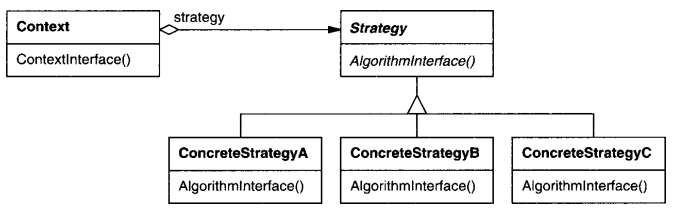
\includegraphics[scale=0.5]{5_padroes-contexto-funcional/5.3_comportamentais/5.3.9_strategy/diagram.png}
	\end{center}
\end{figure}

Exemplo Orientado a Objetos:

\begin{lstlisting}[caption={Strategy Orientação a Objetos},label=oostrategy]
    
    trait Strategy {
        def algorithmInterface() : Unit
    }

    class ConcreteStrategyA() extends Strategy {
        def algorithmInterface() : Unit = {

        }
    }

    class ConcreteStrategyB() extends Strategy {
        def algorithmInterface() : Unit = {

        }
    }

    class Context(var strategy : Strategy) {
        def setStrategy(strategy : Strategy) = this.strategy = strategy

        def contextInterface() : Unit = {
            this.strategy.algorithmInterface()
        }
    }

\end{lstlisting}

Contexto Funcional:

No contexto funcional, já que existem as funções de alta 
ordem (High-order functions), não é necessário definir 
interfaces ou classes concretas para implementar os 
algoritmos: Basta que a função desejada exista e ela 
pode ser passada por parâmetro para a operação 
ContextInterface.

\begin{lstlisting}[caption={Strategy Orientação a Objetos},label=oostrategy]
    
    def algorithmInterfaceA() : Unit = {
        
    }

    def algorithmInterfaceB() : Unit = {
        
    }

    def ContextInterface(algorithmInterface : () => Unit) : Unit = algorithmInterface()

\end{lstlisting}